\clearpage
% \setcounter{page}{1}
% \maketitlesupplementary

\begin{appendices}
\section{Structured Captions}
\label{app:structured-json}

In this section we describe our structured captioning strategy. 
Each caption is a long, detailed JSON that decomposes the image into interpretable fields, covering the objects, background, lighting, aesthetics, photographic attributes, style, and text. This structure guarantees full semantic coverage and improves controllability during training and inference.
The structure of our JSON is described in Table~\ref{tab:JSON-structure}.\begin{table*}[t]
\small
\setlength{\tabcolsep}{6pt}
\renewcommand{\arraystretch}{1.02}
\centering
\begin{tabularx}{\textwidth}{@{}p{3.9cm}p{2.4cm}X@{}}
\toprule
\textbf{Field} & \textbf{Type} & \textbf{Description} \\
\midrule
\texttt{short\_description} & String & A short summary of the image content. \\

\texttt{objects} & Array of Objects &
List of prominent objects. For each object, we record the following fields:
a detailed \texttt{description} of the object, the object's \texttt{location}, \texttt{relative\_size}, \texttt{shape\_and\_color}, \texttt{texture} (opt.), \texttt{appearance\_details} (opt.),
\texttt{relationship} with other objects, and the object's \texttt{orientation} (opt.).
When a human is described, the following fields are also included: the human's \texttt{pose} (opt.), \texttt{expression} (opt.), \texttt{clothing} (opt.), \texttt{action} (opt.), \texttt{gender} (opt.) and \texttt{skin\_tone\_and\_texture} (opt.).
If the image is a cluster of objects then also includes the
\texttt{number\_of\_objects} (opt.).\\

\texttt{background\_setting} & String &
Description of the environment/background. \\

\texttt{lighting} & Object &
Illumination details, including
\texttt{conditions} (e.g., daylight, studio),
\texttt{direction} (key-light orientation), and
\texttt{shadows} (opt.). \\

\texttt{aesthetics} & Object &
Global visual properties, including
\texttt{composition} (e.g., rule of third, symmetrical),
\texttt{color\_scheme} (dominant palette) and
\texttt{mood\_atmosphere} (emotional tone). \\

\shortstack[l]{\texttt{photographic\_}\\\texttt{characteristics}} & Object (optional) &
Camera/focus parameters:
\texttt{depth\_of\_field},
\texttt{focus},
\texttt{camera\_angle}, and
\texttt{lens\_focal\_length}. \\

\texttt{style\_medium} & String &
Artistic/rendering medium (e.g., photograph, oil painting, 3D render). \\

\texttt{text\_render} & Array of Objects &
A list of prominent text renders in the image. For each text render it includes the
\texttt{text},
\texttt{location},
\texttt{size},
\texttt{color},
\texttt{font} and
\texttt{appearance\_details} (opt.). \\

\texttt{context} & String & Additional context that helps understand the image better. \\

\texttt{artistic\_style} & String & High-level artistic/stylistic description (e.g., cinematic, minimalism). \\
\bottomrule
\end{tabularx}
\caption{\textbf{Structure of the JSON-based captions.} Each field captures a distinct aspect of the image, ensuring semantic completeness and consistency.}
\label{tab:JSON-structure}
\end{table*}
 

Our structured captions are generated using Gemini 2.5 with a dedicated system prompt (see Table~\ref{tab:system_prompt}) and using Gemini's structured outputs configured with our JSON schema (see Table~\ref{tab:strcutured_outputs}) that enforce completeness, consistency, and adherence to the predefined schema. 
\begin{table*}[t]
\centering
\begin{tcolorbox}[
    colback=gray!3,
    colframe=gray!30,
    sharp corners,
    left=3pt,right=3pt,top=2pt,bottom=2pt,  % tighter padding
    before skip=2pt, after skip=2pt,        % tighter vertical spacing around box
    fontupper=\ttfamily\scriptsize,         % smaller font (try \tiny if needed)
]
You are a meticulous and perceptive Visual Art Director working for a leading Generative AI company. Your expertise lies in analyzing images and extracting detailed, structured information.
Your primary task is to analyze provided images and generate a comprehensive JSON object describing them. Adhere strictly to the following structure and guidelines:

The output MUST be ONLY a valid JSON object. Do not include any text before or after the JSON object (e.g., no "Here is the JSON:", no explanations, no apologies).

IMPORTANT: When describing human body parts, positions, or actions, always describe them from the PERSON'S OWN PERSPECTIVE, not from the observer's viewpoint. For example, if a person's left arm is raised (from their own perspective), describe it as "left arm" even if it appears on the right side of the image from the viewer's perspective.


The JSON object must contain the following keys precisely:

1. \textbf{`short\_description`}: (String) A concise summary of the image content, 200 words maximum.

2. \textbf{`objects`}: (Array of Objects) List a maximum of 5 prominent objects if there are more than 5, list them in the background. For each object, include:

\quad    * \textbf{`description`}: (String) A detailed description of the object, 100 words maximum.
    
\quad    * \textbf{`location`}: (String) E.g., "center", "top-left", "bottom-right foreground".
    
\quad    * \textbf{`relative\_size`}: (String) E.g., "small", "medium", "large within frame".
    
\quad    * \textbf{`shape\_and\_color`}: (String) Describe the basic shape and dominant color.
    
\quad    * \textbf{`texture`}: (String) E.g., "smooth", "rough", "metallic", "furry".
    
\quad    * \textbf{`appearance\_details`}: (String) Any other notable visual details.
    
\quad    * \textbf{`relationship`}: (String) Describe the relationship between the object and the other objects in the image.
    
\quad    * \textbf{`orientation`}: (String) Describe the orientation or positioning of the object, e.g., "upright", "tilted 45 degrees", "horizontal", "vertical", "facing left", "facing right", "upside down", "lying on its side".
    
If the object is a human or human-like entity, include:

\quad * \textbf{`pose`}: (String) Describe the body position.

\quad * \textbf{`expression`}: (String) Describe facial expression and emotion. E.g., "winking", "joyful", "serious", "surprised", "calm".

\quad        * \textbf{`clothing`}: (String) Describe attire.

\quad        * \textbf{`action`}: (String) Describe the action of the human.

\quad        * \textbf{`gender`}: (String) Describe the gender of the human.
        
\quad        * \textbf{`skin\_tone\_and\_texture`}: (String) Describe the skin tone and texture.

        
If the object is a cluster of objects, include the following:

\quad        * \textbf{`number\_of\_objects`}: (Integer) The number of objects in the cluster.


3. \textbf{`background\_setting`}: (String) Describe the overall environment, setting, or background, including any notable background elements that are not part of the objects section.


4. \textbf{`lighting`}: (Object)

\quad    * \textbf{`conditions`}: E.g., "bright daylight", "dim indoor", "studio lighting", "golden hour".
    
\quad    * \textbf{`direction`}: E.g., "front-lit", "backlit", "side-lit from left".
    
\quad    * \textbf{`shadows`}: Describe the presence of shadows.

5. \textbf{`aesthetics`}: (Object)

\quad    * \textbf{`composition`}: E.g., "rule of thirds", "symmetrical", "centered", "leading lines".

\quad    * \textbf{`color\_scheme`}: E.g., "monochromatic blue", "warm complementary colors", "high contrast".

\quad    * \textbf{`mood\_atmosphere`}: E.g., "serene", "energetic", "mysterious", "joyful".

6. \textbf{`photographic\_characteristics`}: (Object)

\quad    * \textbf{`depth\_of\_field`}: (String) E.g., "shallow", "deep", "bokeh background".

\quad    * \textbf{`focus`}: (String) E.g., "sharp focus on subject", "soft focus", "motion blur".

\quad    * \textbf{`camera\_angle`}: (String) E.g., "eye-level", "low angle", "high angle", "dutch angle".

\quad    * \textbf{`lens\_focal\_length`}: (String) E.g., "wide-angle", "telephoto", "macro", "fisheye".

7. \textbf{`style\_medium`}: (String) Identify the artistic style or medium (e.g., "photograph", "oil painting", "watercolor", "3D render", "digital illustration", "pencil sketch") If the style is not "photograph", but artistic, please describe the specific artistic characteristics under 'artistic\_style', 50 words maximum.

8. \textbf{`artistic\_style`}: (String) Describe specific artistic characteristics, 3 words maximum.

9. \textbf{`context`}: (String) Provide any additional context that helps understand the image better. This should include a general description of the type of image (e.g., Fashion Photography, Product Shot, Magazine Cover, Nature Photography, Art Piece, etc.), as well as any other relevant contextual information that situates the image within a broader category or intended use. For example: "This is a high-fashion editorial photograph intended for a magazine spread"

10. \textbf{`text\_render`}: (Array of Objects) List of a maximum of 5 most prominent text renders in the image. For each text render, include:

\quad    * \textbf{`text`}: (String) The text content.
    
\quad    * \textbf{`location`}: (String) E.g., "center", "top-left", "bottom-right foreground".
    
\quad    * \textbf{`size`}: (String) E.g., "small", "medium", "large within frame".
    
\quad    * \textbf{`color`}: (String) E.g., "red", "blue", "green".
    
\quad    * \textbf{`font`}: (String) E.g., "realistic", "cartoonish", "minimalist".
    
\quad    * \textbf{`appearance\_details`}: (String) Any other notable visual details.

Ensure the information within the JSON is accurate, detailed where specified, and avoids redundancy between fields.
\end{tcolorbox}
\caption{System prompt used to generate structured captions.}
\label{tab:system_prompt}
\end{table*}

\input{tables/JSON_gemini_strcture_output}





\section{Additional Training Details}\label{sec:additional-training-details}

The data distribution is illustrated in Figure~\ref{fig:data_distribution}.
\begin{figure*}[t]
    \centering
    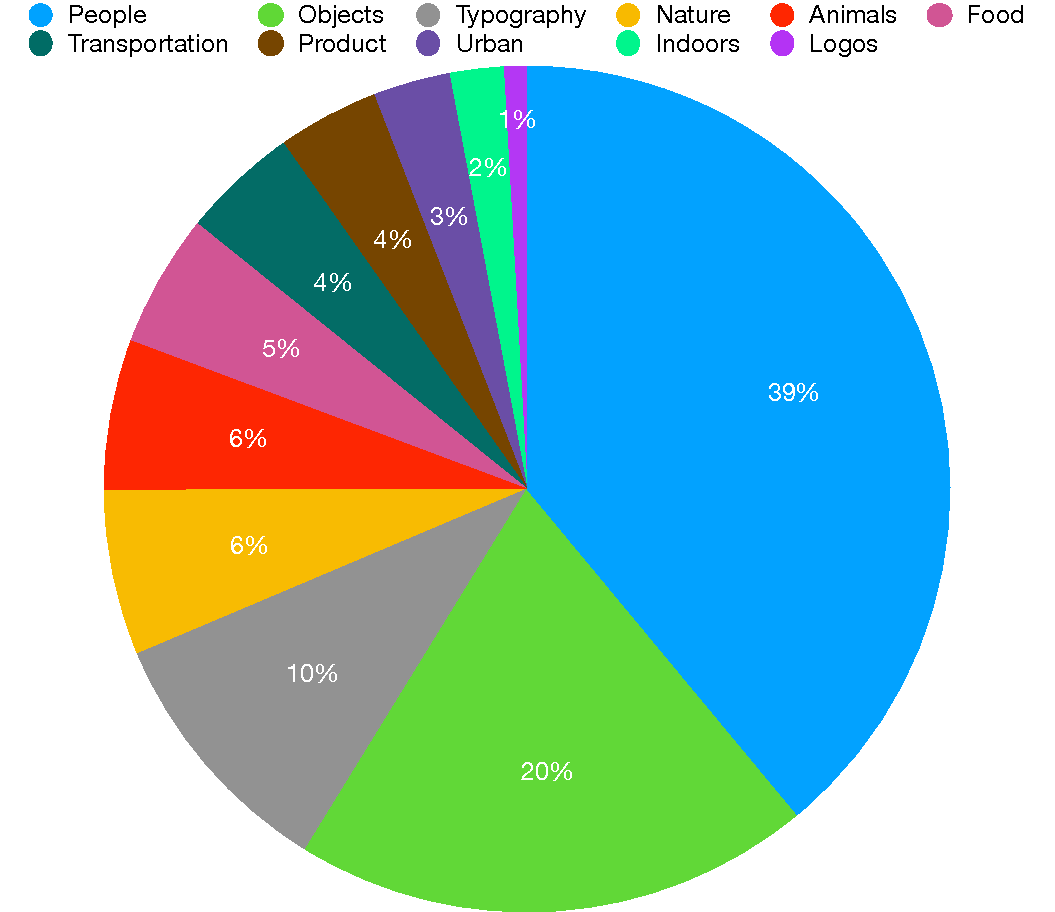
\includegraphics[width=0.6\textwidth]{Figures/data_distribution/data_distribution_good_colors.pdf}
    \vspace{-3mm}
    \caption{\textbf{Data distribution across categories.} 
    People and objects dominate the dataset (39\% and 20\%, respectively), followed by typography (10\%), nature (6\%), animals (6\%), food (5\%), transportation (4\%), product (4\%), urban scenes (3\%), indoors (2\%), and logos (1\%).}
    \label{fig:data_distribution}
    \vspace{-2mm}
\end{figure*}



We train the model using the AdamW optimizer~\cite{loshchilov2017decoupled} with weight decay of $1\times10^{-4}$, $\beta_1=0.9$, $\beta_2=0.999$, and $\epsilon=1\times10^{-15}$. The learning rate is set to $1\times10^{-4}$ with a constant schedule and a warmup of $10$K steps, followed by an additional $2.5$K warmup steps when increasing resolution. Training follows the flow-matching formulation~\cite{lipman2023flowmatchinggenerativemodeling}, with a logit-normal noise schedule combined with resolution-dependent timestep shifting~\cite{esser2024scaling}.


We train the model in stages of increasing resolution. The first stage is conducted at $256^2$ resolution for $652$k steps, where the initial $300$k steps employ REPA~\cite{yu2024representation} using DINOv2-L encodings~\cite{oquab2023dinov2} and REPA coefficient of 0.1. Training then continues for an additional $100$k steps at $512^2$ resolution, followed by $50$k steps at $1024^2$. At each resolution stage, the effective batch size starts at approximately $1$K and is gradually increased to $2$K as training progresses.

Post-training, we perform aesthetic finetuning with 3,000 hand-picked images, followed by DPO training~\cite{wallace2024diffusion} with dynamic beta~\cite{liu2025improving} to improve text rendering.





\section{Additional Ablation Studies Details}
\label{sec:appendix_ablation}

We provide implementation details for the ablation studies discussed in Section~\ref{sec:captions} (long structured captions vs. short captions) and Section~\ref{sec:dimfusion} (convergence behavior across architectures).
To reduce compute cost, all ablations were conducted under identical training and sampling conditions using 1B-parameter models trained with the SDXL VAE \cite{podell2023sdxl}.
Table \ref{tab:ablations_model_arch} lists the architectural hyperparameters used in all experiments.
\begin{table}[H]
  \centering
  \footnotesize
  \begin{tabular}{cccccc}
    \toprule
    \textbf{\makecell{Dual-stream \\ Blocks}} &
    \textbf{\makecell{Single-stream \\ Blocks}} &    
    \textbf{\makecell{FFN \\ Dimension}} &
    \textbf{\makecell{Attention \\ Heads}} &
    \textbf{\makecell{Head dim}} &
    $\left(d_t, d_h, d_w\right)$ \\
    \midrule
    8 & 20 & 6144 & 24 & 64 & $(4,\,30,\,30)$ \\
    \bottomrule
  \end{tabular}
  \caption{Model configuration for the 1B-parameter models used in the ablation studies. Each model is trained under identical conditions, differing only by caption type (long vs. short) or architectural variant (Baseline, DimFusion, TokenFusion).}
  \label{tab:ablations_model_arch}
\end{table}


In Section \ref{sec:captions}, we examine the effect of caption length using the \emph{DimFusion} architecture with \emph{SmolLM3-3B} as the LLM, trained once with long structured captions and once with short captions.
In Section \ref{sec:dimfusion}, we compare three architectures trained on long structured captions.
The baseline follows \cite{esser2024scaling} and uses T5 \cite{raffel2020exploring} as the text encoder.
We further evaluate two large-language-model fusion variants that share the same hyperparameters as the baseline:
(1) \emph{DimFusion} with \emph{SmolLM3-3B} as the LLM; and
(2) \emph{TokenFusion}, following HiDream \cite{cai2025hidream}, concatenates SmolLM3-3B hidden states with the text embeddings along the \emph{sequence} dimension, effectively doubling the number of text tokens in each attention layer.

All models were trained on 70M licensed image-caption pairs, with the same optimizer, learning rate and noise scheduling described in Appendix~\ref{sec:additional-training-details}, and effective batch size of 1024. We also employed REPA~\cite{yu2024representation} with DINOv2-L encodings~\cite{oquab2023dinov2} and a REPA coefficient of 0.5.
For evaluation, FID was computed on 30K samples from the COCO-2014~\cite{lin2014microsoft} validation split, using 50 inference steps and no classifier-free guidance.


\section{Additional Samples from \modelname{}}

Additional samples from \modelname{} in various aspect ratios appear in Figure~\ref{fig:app_samples}, and additional examples for refinement and disentanglement appear in Figure~\ref{fig:app_disentanglement}.

\newcommand{\ResRow}[4]{%
  \begin{minipage}[t]{0.24\textwidth}\centering
    \includegraphics[width=\linewidth,keepaspectratio]{#1}
  \end{minipage}\hfill
  \begin{minipage}[t]{0.24\textwidth}\centering
    \includegraphics[width=\linewidth,keepaspectratio]{#2}
  \end{minipage}\hfill
  \begin{minipage}[t]{0.24\textwidth}\centering
    \includegraphics[width=\linewidth,keepaspectratio]{#3}
  \end{minipage}\hfill
  \begin{minipage}[t]{0.24\textwidth}\centering
    \includegraphics[width=\linewidth,keepaspectratio]{#4}
  \end{minipage}
}


\begin{figure*}[t]
  \centering
  \setlength{\tabcolsep}{2pt}

  % --- 832x1216 (portrait) ---
  \ResRow{Figures/samples/832x1216/1.jpg}{Figures/samples/832x1216/2.jpg}{Figures/samples/832x1216/3.jpg}{Figures/samples/832x1216/4.jpg}
  \\[8pt]

  % --- 1024x1024 (square) ---
  \ResRow{Figures/samples/1024x1024/1.jpg}{Figures/samples/1024x1024/2.jpg}{Figures/samples/1024x1024/3.jpg}{Figures/samples/1024x1024/4.jpg}
  \\[8pt]

  % --- 1152x896 (landscape) ---
  \ResRow{Figures/samples/1152x896/1.jpg}{Figures/samples/1152x896/2.jpg}{Figures/samples/1152x896/3.jpg}{Figures/samples/1152x896/4.jpg}
  \\[8pt]

  % --- 1216x832 (landscape) ---
  \ResRow{Figures/samples/1216x832/1.jpg}{Figures/samples/1216x832/2.jpg}{Figures/samples/1216x832/3.jpg}{Figures/samples/1216x832/4.jpg}
  \\[8pt]

  \caption{Additional samples from \modelname{} in various aspect ratios.}
  \label{fig:app_samples}
\end{figure*}
\setlength{\tabcolsep}{0.5pt}
\renewcommand{\arraystretch}{1.0}

\begin{figure*}[t]
\centering
\newcommand{\imgw}{0.24\textwidth} % 4 images × 0.24 ≈ full width
\begin{tabular}{@{}cccc@{}}

  % Row 4
  \includegraphics[width=\imgw]{Figures/disentanglement/images_ski/1.jpg} &
  \includegraphics[width=\imgw]{Figures/disentanglement/images_ski/2.jpg} &
  \includegraphics[width=\imgw]{Figures/disentanglement/images_ski/3.jpg} &
  \includegraphics[width=\imgw]{Figures/disentanglement/images_ski/4.jpg}
  \\[-2pt]
  \parbox{\imgw}{\scriptsize\centering \textbf{}} &
  \parbox{\imgw}{\scriptsize\centering \textbf{make snowing}} &
  \parbox{\imgw}{\scriptsize\centering \textbf{move to desert}} &
  \parbox{\imgw}{\scriptsize\centering \textbf{make night}}
  \\[+2pt]

  \includegraphics[width=\imgw]{Figures/disentanglement/images_owl/1.jpg} &
  \includegraphics[width=\imgw]{Figures/disentanglement/images_owl/2.jpg} &
  \includegraphics[width=\imgw]{Figures/disentanglement/images_owl/3.jpg} &
  \includegraphics[width=\imgw]{Figures/disentanglement/images_owl/4.jpg}
  \\[-2pt]

  % Wrapped labels under each image (row)
  \parbox{\imgw}{\scriptsize\centering \textbf{}} &
  \parbox{\imgw}{\scriptsize\centering \textbf{make owl brown}} &
  \parbox{\imgw}{\scriptsize\centering \textbf{owl to lemur}} &
  \parbox{\imgw}{\scriptsize\centering \textbf{add jungle vegetation}}
  \\[+2pt]

    \includegraphics[width=\imgw]{Figures/disentanglement/images_icecream/1.jpg} &
  \includegraphics[width=\imgw]{Figures/disentanglement/images_icecream/3.jpg} &
  \includegraphics[width=\imgw]{Figures/disentanglement/images_icecream/2.jpg} &
  \includegraphics[width=\imgw]{Figures/disentanglement/images_icecream/4.jpg}
  \\[-2pt]

  % Wrapped labels under each image (row)
  \parbox{\imgw}{\scriptsize\centering \textbf{}} &
  \parbox{\imgw}{\scriptsize\centering \textbf{blueberries to strawberries}} &
  \parbox{\imgw}{\scriptsize\centering \textbf{blue to pink}} &
  \parbox{\imgw}{\scriptsize\centering \textbf{add mint leaves}}
  \\[+2pt]

  \includegraphics[width=\imgw]{Figures/disentanglement/images_cup/1.jpg} &
  \includegraphics[width=\imgw]{Figures/disentanglement/images_cup/2.jpg} &
  \includegraphics[width=\imgw]{Figures/disentanglement/images_cup/3.jpg} &
  \includegraphics[width=\imgw]{Figures/disentanglement/images_cup/4.jpg}
  \\[-2pt]

  % Wrapped labels under each image (row)
  \parbox{\imgw}{\scriptsize\centering \textbf{}} &
  \parbox{\imgw}{\scriptsize\centering \textbf{blue cup with flower ornaments}} &
  \parbox{\imgw}{\scriptsize\centering \textbf{add scattered daisies}} &
  \parbox{\imgw}{\scriptsize\centering \textbf{hand steering coffee with teaspoon}}
  \\[+2pt]

    \includegraphics[width=\imgw]{Figures/disentanglement/images_dog/1.jpg} &
  \includegraphics[width=\imgw]{Figures/disentanglement/images_dog/2.jpg} &
  \includegraphics[width=\imgw]{Figures/disentanglement/images_dog/3.jpg} &
  \includegraphics[width=\imgw]{Figures/disentanglement/images_dog/4.jpg}
  \\[-2pt]

  % Wrapped labels under each image (row)
  \parbox{\imgw}{\scriptsize\centering \textbf{}} &
  \parbox{\imgw}{\scriptsize\centering \textbf{black dog}} &
  \parbox{\imgw}{\scriptsize\centering \textbf{light-green coat, hoodie on}} &
  \parbox{\imgw}{\scriptsize\centering \textbf{Add snow}}


\end{tabular}

\vspace{-3pt}
\caption{Additional refinement examples.}
\label{fig:app_disentanglement}
\end{figure*}



% \section{User Study}
% Print screens to demonstrate the user interface for our user study are provided in Figure~\ref{fig:user_study_ui}.

% 
\begin{figure}[t]
\centering


  \includegraphics[width=\linewidth]{Figures/user_study/preference_user_study.jpg}

  \includegraphics[width=\linewidth]{Figures/user_study/tabr_user_study.jpg}


\vspace{-3mm}
\caption{\textbf{User study examples.} 
\textbf{(Top)} and \textbf{(Bottom)} visualizations of the user study conducted for overall preference and TaBR respectively.}
\label{fig:user_study_ui}
\vspace{-2mm}
\end{figure}

\end{appendices}

